\documentclass[11pt]{article}

% Language setting
% Replace `english' with e.g. `spanish' to change the document language
\usepackage[english]{babel}

% Set page size and margins
% Replace `letterpaper' with `a4paper' for UK/EU standard size
\usepackage[letterpaper,top=2cm,bottom=2cm,left=3cm,right=3cm,marginparwidth=1.75cm]{geometry}

% Useful packages
\usepackage{amsmath}
\usepackage{graphicx}
\usepackage[colorlinks=true, allcolors=blue]{hyperref}

\title{Spring 2024 \\
"Identifying Man's best Friend" \\
Project Proposal}
\author{Edward Wang}
\date{}

\begin{document}
\maketitle
\section{Problem Statement}

For centuries, dogs have stood as steadfast companions to humans, earning the endearing title of "man's best friend." This remarkable bond traces back thousands of years. Dogs were domesticated more than 10,000 years ago in Europe \cite{dog1}, with earlier ties in other regions of the world. Initially serving as hunting partners, guardians, and eventually cherished members of the family, dogs have evolved and adapted to various roles and environments. From the loyal sled dogs of the Arctic to the quite literal definition of role by acting in various movies, their versatility and loyalty made them beloved across diverse cultures worldwide. 

Today, dogs are the most popular pet in the U.S., with 65.1 million households  proudly owning a dog \cite{forbes}. That's 1 in every 2 households! The American Kennel Club (AKC) recognizes 200 distinct breeds \cite{akc}, some of which bear striking resemblances to each other despite possessing notably different temperaments. As depicted in Figure \ref{fig:husky}, the Siberian Husky is well known for its stubbornness and independent nature     \cite{akc_husky}, while the Alaskan Malamute, nearly twice its weight, tends to exhibit characteristics more akin to those of a watchdog \cite{akc_mal}. 

\begin{figure}[h]
\centering
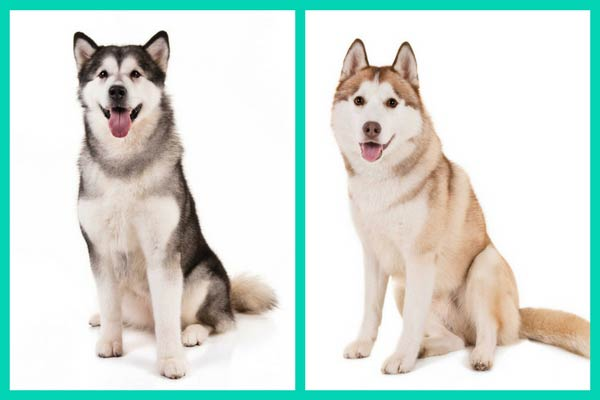
\includegraphics[width=0.25\linewidth]{malamutehusky.jpg}
\caption{\label{fig:husky}Alaskan Malamute (Left) and Siberian Husky (Right)}
\end{figure}

There are various other breeds that are very similar. For example, the Border Collie and Australian Shepherd is another close looking pair. \textbf{The objective is to explore and develop a Neural Network capable of accurately identifying various breeds of dogs.}

\section{Data Collection}

The data source for this project is the Stanford Dogs Dataset \cite{data_source}, which contains images of 120 breeds of dogs from around the world. This dataset is part of the larger ImageNet dataset with annotations and labels. The Stanford Dogs Dataset contains colored images of dogs in various poses and locations. 

In line with computational constraints, I will opt to focus on the top 20 popular dog breeds for this analysis. Certain breeds that deviate from the archetype of a traditional family pet, such as the African Hunting Dog and Dingo, are deliberately excluded from the dataset.Some breeds may be aggregated together to streamline the dataset and ensure equal class representation. Moreover, where image availability is limited, additional data will be collected through web scraping from Google Images.

\section{Proposed Methodology}

\subsection{Data preparation}  

The Stanford Dog Dataset contains images of various sizes, thus, my initial data preparation will involve resizing all images to a standardized resolution. I will opt for a resolution of 300x300 pixels as a starting point in order to balance computational efficiency with image clarity. However, if initial training times prove to be too long, I will downsize the images further to 150x150 pixels.

Next, the images will be converted to gray-scale to remove any color biases and help the neural network generalize across various colors. This will further help reduce our training time by changing the dimension of the dataset from 300x300x3, where 3 represents the colored dimensions RGB to just 300x300x1 where 1 represents the gray-scale. This will fully prepare our dataset for training.   

The number of images per class is crucial for maintaining robust model performance. By verifying the distribution of images across classes, I can address potential biases and take appropriate step, such as obtaining additional images, to mitigate them. 

Finally, to prevent over fitting, I will use image augmentation to artificially create additional training images. This includes randomly tilting the image, flipping on the horizontal axis, adjusting hue and contrast, or even adding blur. 

\subsection{Modeling}

The objective is to identify the various breeds of dogs, so the best model would be a image classification model. Specifically, I will be using a Convolutional Neural Network (CNN). CNN is a Deep Learning Neural Network that can take in an input image, assign the weights and biases, and produce a final prediction.  

Unlike a traditional Neural Network, a Convoluational Neural Network contains Convoluational layers as the name implies. The convolutional layers are responsible for feature extraction process. These layers consist of filters, or kernels, that capture relevant features and patterns of the input image. These layers help detect the edges, textures, shapes, and other aspects unique to the image. For example, in a simple example of identifying a slice of pie vs a whole pie, the CNN would learn the unique triangle shape of the slice vs the round circle of a whole pie. In the dog dataset, this would akin to the length of the fur, length of the snout, or how the head and tail are shaped. 

One process to speed up training and improve accuracy is to leverage transfer learning. Transfer learning is the process of using the pre-trained CNN as a starting point and fine-tuning it on the new dataset. Essentially, this fine-tuning process is training the last few layers of the CNN on the new dataset. Some of the major pre-trained CNNs on larger image datasets are ResNet, VGG16, Inception-v3, and MobileNet.

\section{Proposed Evaluation}   

During training, I will monitor both loss and accuracy metrics to gauge the model's training progress. Loss indicates how well the model is fitting the training data, while accuracy measures the proportion of correctly classified instances. These metrics collectively help in determining if the learning rate is appropriate and if further training epochs are necessary for optimal model performance.

I will primarily utilize the F1-Score to assess the final performance of the different models. The F1-Score offers a balanced evaluation by considering both precision and recall. Precision evaluates the model's capability to avoid false positives, while recall measures its ability to identify all positive instances. 

I can also consider precision, quality of a positive prediction made by the model, depending on the use case. For example, if this model was deployed at an animal shelter, a high precision ensures that the shelter staff can be confident in the breed information provided by the model when presenting dogs to potential adopters. This minimizes the risk of misinforming adopters about the dog's breed, which could lead to disappointment or misalignment with the adopter's preferences.

\bibliographystyle{alpha}
\bibliography{sample}

\end{document}